\documentclass[aspectratio=169]{beamer}
\usepackage[utf8]{inputenc}
\usepackage[T1]{fontenc}
\usepackage[portuguese]{babel}
\usepackage{graphicx}
\usepackage{helvet}



\usepackage{amsmath, amsthm, amsfonts, amscd}
\usepackage{tikz}
\usepackage{tikz-cd}
\usepackage{amssymb}
\usepackage{listings}
\usepackage{xcolor}


\usepackage[backend=biber, style=authoryear]{biblatex}

\addbibresource{refs.bib}


\usetheme[mode=light]{sthlmnord}

%\setbeamertemplate{navigation symbols}{}
%\setbeamercolor{background canvas}{bg=white}
%\setbeamercolor{title}{fg=black}
%\setbeamercolor{frametitle}{fg=black}
%\setbeamerfont{frametitle}{size=\Large, series=\bfseries}



% Define custom styles for clarity
\tikzset{
    % General settings for the tree
    every node/.style={
        draw, % Draw a border around nodes
        shape=circle, % Circular shape for all nodes
        minimum size=1cm, % Consistent size for easier readability
        inner sep=0pt, % Adjust inner spacing
        font=\large\bfseries % Standard large, bold font
    },
    % Specific styles for operator nodes (internal nodes)
    operator/.style={
        minimum size=1cm, % Optional: you could adjust this if needed
        fill=white % Keep background white or define a color
    },
    % Specific styles for operand nodes (leaf nodes)
    operand/.style={
        font=\large, % Revert font style (no bold)
        fill=white
    },
    % Style for the connecting edges
    edge/.style={
        thick,
        - % Simple straight edges without arrows
    }
}

%pseudo-code
\lstset{
    basicstyle=\ttfamily\footnotesize, % Fonte monoespaçada e legível
    keywordstyle=\color{blue}\bfseries,
    commentstyle=\color{gray}\itshape,
    breaklines=true,
    showstringspaces=false,
    tabsize=2,
    extendedchars=true,
    % Suporte para acentos em português dentro do listings
    literate={á}{{\'a}}1 {ã}{{\~a}}1 {ç}{{\c{c}}}1 {õ}{{\~o}}1 {í}{{\'i}}1 {ú}{{\'u}}1 {é}{{\'e}}1 {Ç}{{\c{C}}}1 {Õ}{{\~O}}1 {Ã}{{\~A}}1 {É}{{\'E}}1
}

\setbeamertemplate{title page}{
	\vfill
	\begin{centering}
		{\usebeamerfont{title}\usebeamercolor[fg]{title}\Huge \textbf{\inserttitle}}\par
		\vspace{1cm}
		{\usebeamerfont{author}\large \insertauthor}\par
	\end{centering}
	\vfill
	\begin{center}
		
\includegraphics[height=1.6cm]{../figures/logo_unespar.png} \hfill
		
\includegraphics[height=1.2cm]{../figures/logo_evento.png} \hfill
		
\includegraphics[height=1.2cm]{../figures/mat.png} \hfill
		
\includegraphics[height=1.2cm]{../figures/prpgem.png}
	\end{center}
	\vspace{0.2cm}
}

\setbeamertemplate{footline}{
	\ifnum\insertframenumber>1
	\hbox{%
		\begin{beamercolorbox}[wd=.8\paperwidth,ht=1cm,dp=0.5cm,leftskip=1cm]{}
			\scriptsize\color{gray} X Ágora Matemática – Unespar, campus de Campo Mourão
		\end{beamercolorbox}%
		\begin{beamercolorbox}[wd=.2\paperwidth,ht=1cm,dp=0.5cm,right,rightskip=0.8cm]{}
			
\includegraphics[height=1.2cm]{../figures/logo_evento.png}
		\end{beamercolorbox}%
	}
	\fi
}

%Página de título
\title{Teorema da Base de Hilbert}
\author{\Large
	Wallace Carlos Rodrigues \\
	Rodrigo Eber de Almeida \\
	Lucas Gabriel da Silveira Ames \\
	João Paulo Chiari de Gasperi \\
}
\date{}


\begin{document}

% Capa
\begin{frame}[plain]
	\titlepage
\end{frame}

\begin{frame}{Conteúdo}
	\tableofcontents
\end{frame}

\section{Funcionamento do Jogo}

\begin{frame}{Regras}
	\begin{block}{Regras}
		\begin{enumerate}
			\item Você recebe quatro números aleatórios (Entre 1 e 13);
			\item Você pode usar adição, subtração, multiplicação e divisão;
			\item O resultado final da conta deve ser 24;
			\item Cada número disponível só pode ser usado uma vez.
		\end{enumerate}
	\end{block}
\end{frame}

\begin{frame}{Valores das cartas}
	\begin{center}
		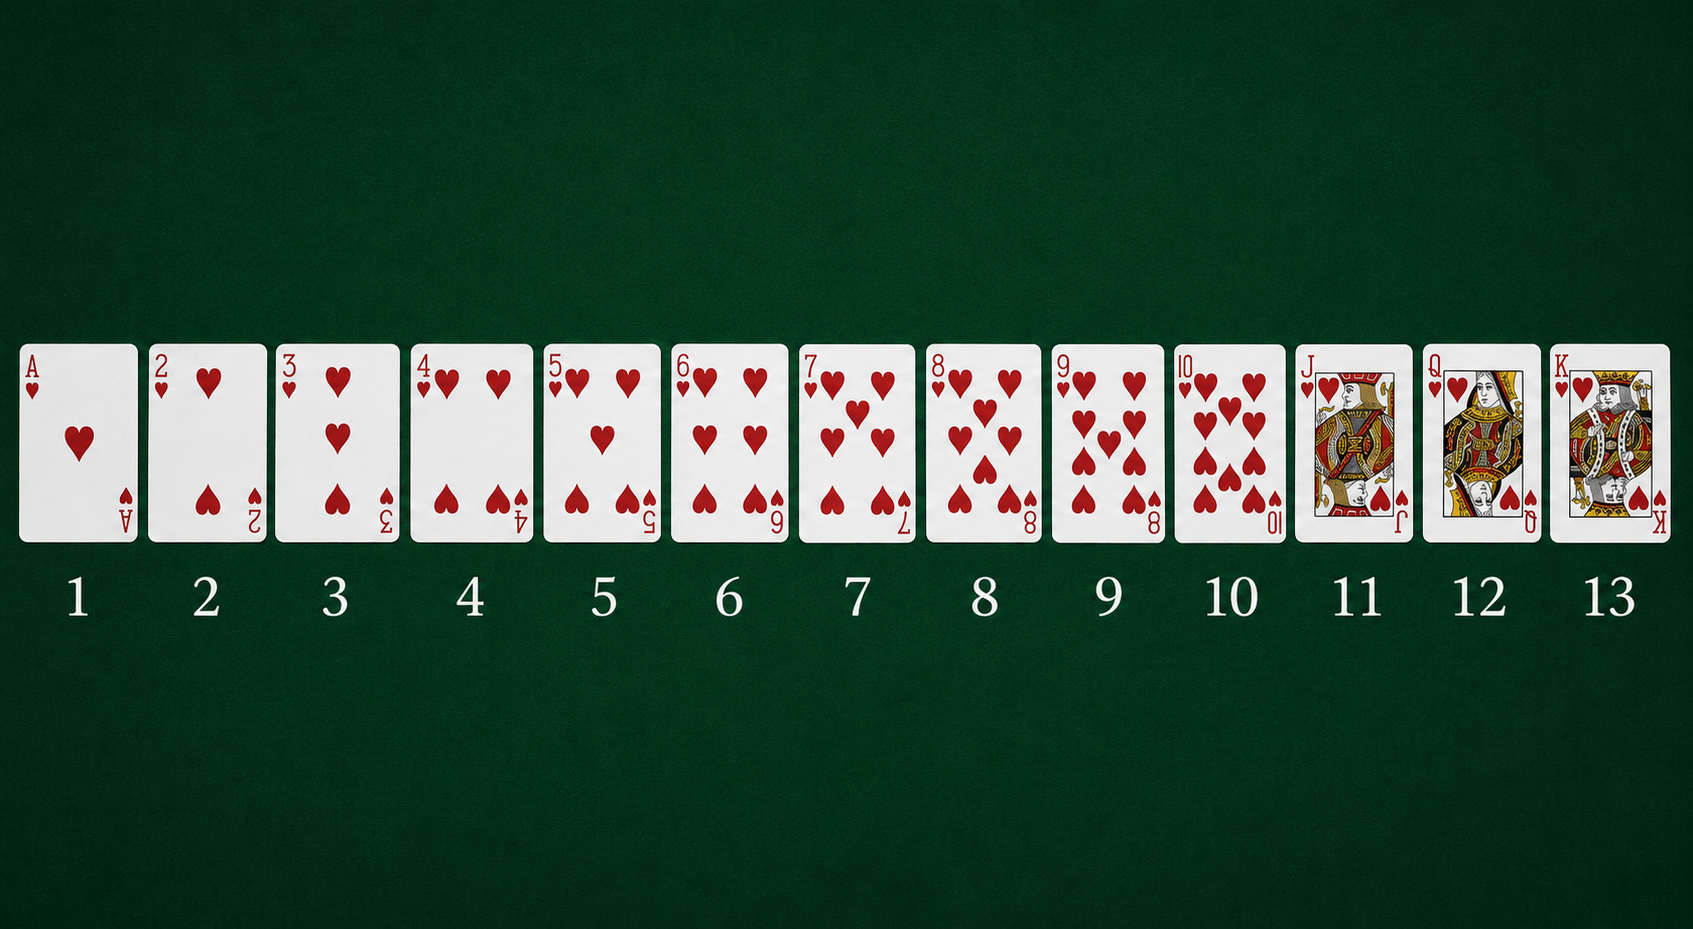
\includegraphics[height=0.9\textheight]{../figures/cards.png}
	\end{center}
\end{frame}

\begin{frame}{Exemplo}
	\begin{center}
		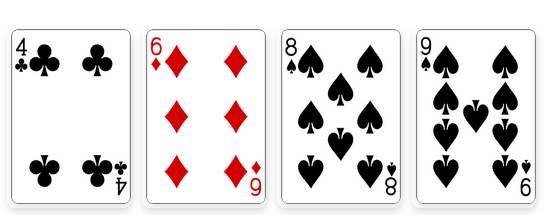
\includegraphics[height=0.6\textheight]{../figures/exemplo.png}
	\end{center}
	\pause
	\begin{alertblock}{Solução}
		$(4*6)*(9-8)$
	\end{alertblock}
\end{frame}

\begin{frame}{Métodos}
	\begin{block}{Método da Alavanca}
		Realizado quando uma das cartas é divisora de $24$.
		\begin{itemize}
			\item Escolhemos um divisor de $24$, digamos $n$;
			\item Tentamos utilizar as outras $3$ cartas para formar $\frac{24}{n}$;
			\item Multiplicamos $n$ por $\frac{24}{n}$, obtendo o número $24$.
		\end{itemize}
	\end{block}
\end{frame}

\begin{frame}{Exemplo}
	\begin{center}
		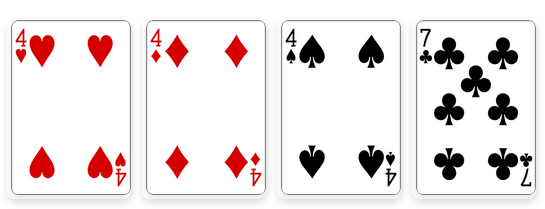
\includegraphics[height=0.6\textheight]{../figures/exemplo_alavanca.png}
	\end{center}
	\pause
	\begin{alertblock}{Solução}
		$4*(7-(4/4))$
	\end{alertblock}
\end{frame}


\section{Análise e implementação computacional}

\begin{frame}{Quantidade de Jogos}
	\begin{itemize}
		\item O baralho tem 52 cartas, onde seus valores variam de 1 a 13 e se repetem 4 vezes;
		      \pause
		\item Queremos contar de quantas formas diferentes podemos selecionar 4 elementos do conjunto $\{1, 2, ..., 13\}$, permitindo a repetição;
		      \pause
		\item Utilizamos a fórmula da combinação com repetição: $$C(n,k)=\frac{(n+k-1)!}{k!(n-1)!};$$
		      \pause
		\item Obtemos que a quantidade todal de jogos possíveis é $$1820.$$
	\end{itemize}
\end{frame}

\begin{frame}{Árvore de Expressões}
	\begin{center}
		$(3+5)*(10-2)$
	\end{center}
	\pause
	\begin{center}
		\begin{tikzpicture}
			% Root node
			\node [operator] (root) at (0,0) {*};

			% Left sub-tree
			\node [operator] (plus) at (-3,-2.5) {+};
			\node [operand] (three) at (-4,-5) {3};
			\node [operand] (five) at (-2,-5) {5};

			% Right sub-tree
			\node [operator] (minus) at (3,-2.5) {-};
			\node [operand] (ten) at (2,-5) {10};
			\node [operand] (two) at (4,-5) {2};

			% Connecting lines with simplified "edge" style
			% The labels illustrate the left and right pointers conceptually, 
			% though the connection is simple and does not contain extra logic in this drawing.
			\draw [edge] (root) -- (plus) node[midway, left, draw=none, shape=rectangle, minimum size=0pt, font=\normalsize, xshift=-0.2cm, yshift=0.3cm] {Left};
			\draw [edge] (root) -- (minus) node[midway, right, draw=none, shape=rectangle, minimum size=0pt, font=\normalsize, xshift=0.2cm, yshift=0.3cm] {Right};

			\draw [edge] (plus) -- (three) node[midway, left, draw=none, shape=rectangle, minimum size=0pt, font=\normalsize, xshift=-0.1cm, yshift=0.2cm] {};
			\draw [edge] (plus) -- (five) node[midway, right, draw=none, shape=rectangle, minimum size=0pt, font=\normalsize, xshift=0.1cm, yshift=0.2cm] {};

			\draw [edge] (minus) -- (ten) node[midway, left, draw=none, shape=rectangle, minimum size=0pt, font=\normalsize, xshift=-0.1cm, yshift=0.2cm] {};
			\draw [edge] (minus) -- (two) node[midway, right, draw=none, shape=rectangle, minimum size=0pt, font=\normalsize, xshift=0.1cm, yshift=0.2cm] {};
		\end{tikzpicture}
	\end{center}
\end{frame}

\begin{frame}[fragile]{Estrutura de Dados: Classe Expressão}
	\begin{lstlisting}[mathescape=true]
CLASSE Expressão:
    ATRIBUTO esquerda: Expressão
    ATRIBUTO operação: Texto
    ATRIBUTO direita: Expressão

    MÉTODO Avaliar() RETORNA Número Decimal:
        // Executa o cálculo da árvore de expressões
        // Ex: calcula (esquerda + direita)
        ...

    MÉTODO Ordenar():
        // Organiza a ordem dos nós da árvore
        // Ex: garante que o maior valor fique à esquerda
        ...
\end{lstlisting}
\end{frame}

% ---- SLIDE 1: CASOS BASE (1, 2 e 3 Cartas) ----
\begin{frame}[fragile]{Algoritmo: Solucionador Recursivo (Parte 1)}
	\begin{lstlisting}[mathescape=true]
FUNÇÃO EncontrarSoluções(Cartas):
    CRIAR lista vazia de Soluções

    SE número de Cartas == 1:
        ADICIONAR a Carta às Soluções
    
    SE número de Cartas == 2:
        ADICIONAR todas as operações possíveis entre as Cartas

    SE número de Cartas == 3:
        PARA CADA par possível de Cartas:
            CartaRestante = a 1 carta fora do par
            ResultadosDoPar = EncontrarSoluções(Par) // Recursão

            PARA CADA Res em ResultadosDoPar:
                ADICIONAR EncontrarSoluções(Res, CartaRestante)
\end{lstlisting}
\end{frame}


% ---- SLIDE 2: CASO COMPLEXO (4 Cartas) e FILTRO ----
\begin{frame}[fragile]{Algoritmo: Solucionador Recursivo (Parte 2)}
	\begin{lstlisting}[mathescape=true]
    SE número de Cartas == 4:
        // Estratégia A: Agrupar em 3 e 1
        PARA CADA grupo de 3 Cartas:
            CartaRestante = a 1 carta que sobrou
            ResGrupo = EncontrarSoluções(Grupo de 3) // Recursão

            PARA CADA Res em ResGrupo:
                ADICIONAR EncontrarSoluções(Res, CartaRestante)

        // Estratégia B: Agrupar em dois pares (2 e 2)
        PARA CADA par de Cartas:
            ParRestante = as outras 2 cartas
            Res1 = EncontrarSoluções(Primeiro Par)  // Recursão
            Res2 = EncontrarSoluções(ParRestante)    // Recursão

            PARA CADA r1 em Res1:
                PARA CADA r2 em Res2:
                    ADICIONAR EncontrarSoluções(r1, r2)

    RETORNAR Soluções
\end{lstlisting}
\end{frame}

\begin{frame}{Resultados}
	\begin{block}{Total}
		$1362$ ou $74,8\%$ dos jogos possui solução;
	\end{block}

	\begin{block}{Alavanca}
		Desses, $1362$ ou $74,8\%$ dos jogos possui solução utilizando o método alavanca;
	\end{block}
\end{frame}

\begin{frame}{Objetivos Futuros}
	\begin{enumerate}
		\item Buscar por outros métodos e verificar a eficiência;
		\item Estabelecer uma ordem de estratégia ótima;
		\item Tentar formalizar e demonstrar os resultados alcançados analíticamente.
	\end{enumerate}
\end{frame}



\begin{frame}{Referências}
	\nocite{*}
	\printbibliography
\end{frame}

\end{document}